\chapter{Phase 1: Binary baselines, calibration and ensembling}
\label{ch:phase1}

% ~12-15 pages

\section{Per-model accuracy with confidence intervals}
% Reference table:
% % Auto-generated by master/generate_thesis_tables.py
% Do not edit by hand — re-run the generator instead.
\begin{table}[t]
  \centering
  \caption{Per-model test performance with bootstrap 95\% confidence intervals on the held-out test set ($N = 550$). ECE is reported before and after temperature scaling fit on the validation set.}
  \label{tab:phase1-summary}
  \small
  \begin{tabular}{lcccccc}
    \toprule
    Model & Test acc (\%) & 95\% CI & AUC & ECE raw & ECE TS & $T$ \\
    \midrule
    ResNet50 & 95.27 & [93.45, 97.09] & 0.9888 & 0.0199 & 0.0182 & 1.19 \\
Xception & 95.45 & [93.82, 97.09] & 0.9852 & 0.0174 & 0.0224 & 1.16 \\
DenseNet121 & 95.64 & [94.00, 97.27] & 0.9919 & 0.0288 & 0.0269 & 1.03 \\
VGG16 & 95.64 & [94.00, 97.27] & 0.9900 & 0.0255 & 0.0153 & 1.44 \\
CNN & 96.00 & [94.36, 97.45] & 0.9867 & 0.0317 & 0.0317 & 1.00 \\
CNN (Tanh+ReLU) & 92.91 & [90.72, 94.91] & 0.9699 & 0.0460 & 0.0415 & 1.21 \\
    \bottomrule
  \end{tabular}
\end{table}

%
% Discuss:
% - All 5 strong models cluster in 95-96\% — visualised in
%   \cref{fig:phase1-acc-ci}.
% - Boostrap 95\% CIs overlap heavily for the top 5; the CNN
%   (Tanh+ReLU) variant is clearly worse.
% - The custom CNN slightly leads (96\%), surprising given its smaller
%   parameter count. Likely due to grayscale preprocessing matching the
%   training distribution.
%
% \begin{figure}[t]
%   \centering
%   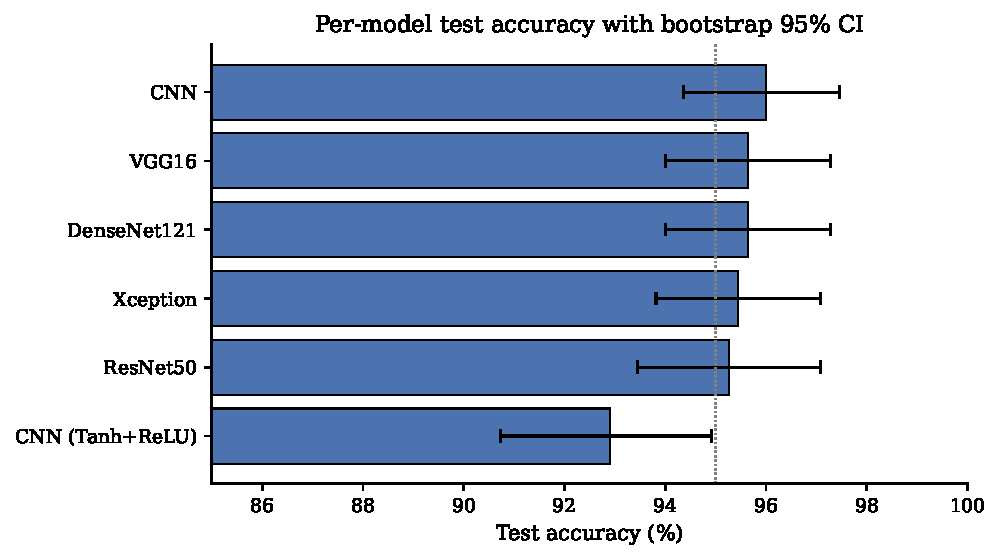
\includegraphics[width=0.85\linewidth]{figures/fig_phase1_accuracy_ci.pdf}
%   \caption{Per-model test accuracy with bootstrap 95\% CI.}
%   \label{fig:phase1-acc-ci}
% \end{figure}

% Auto-generated by master/generate_thesis_tables.py
% Do not edit by hand — re-run the generator instead.
\begin{table}[t]
  \centering
  \caption{Per-model test performance with bootstrap 95\% confidence intervals on the held-out test set ($N = 550$). ECE is reported before and after temperature scaling fit on the validation set.}
  \label{tab:phase1-summary}
  \small
  \begin{tabular}{lcccccc}
    \toprule
    Model & Test acc (\%) & 95\% CI & AUC & ECE raw & ECE TS & $T$ \\
    \midrule
    ResNet50 & 95.27 & [93.45, 97.09] & 0.9888 & 0.0199 & 0.0182 & 1.19 \\
Xception & 95.45 & [93.82, 97.09] & 0.9852 & 0.0174 & 0.0224 & 1.16 \\
DenseNet121 & 95.64 & [94.00, 97.27] & 0.9919 & 0.0288 & 0.0269 & 1.03 \\
VGG16 & 95.64 & [94.00, 97.27] & 0.9900 & 0.0255 & 0.0153 & 1.44 \\
CNN & 96.00 & [94.36, 97.45] & 0.9867 & 0.0317 & 0.0317 & 1.00 \\
CNN (Tanh+ReLU) & 92.91 & [90.72, 94.91] & 0.9699 & 0.0460 & 0.0415 & 1.21 \\
    \bottomrule
  \end{tabular}
\end{table}


\section{Statistical significance: McNemar tests}
% Auto-generated by master/generate_thesis_tables.py
% Do not edit by hand — re-run the generator instead.
\begin{table}[t]
  \centering
  \caption{Pairwise McNemar tests on the binary test set ($N = 550$). $b$ counts predictions where A is correct and B wrong; $c$ vice versa. $p < 0.05$ indicates a statistically significant difference in error rates.}
  \label{tab:phase1-mcnemar}
  \scriptsize
  \begin{tabular}{lccccc}
    \toprule
    Comparison & $b$ & $c$ & $\chi^2$ & $p$-value & Significant? \\
    \midrule
    ResNet50 vs Xception & 11 & 12 & 0.00 & 1.0000 & No \\
ResNet50 vs DenseNet121 & 8 & 10 & 0.06 & 0.8137 & No \\
ResNet50 vs VGG16 & 5 & 7 & 0.08 & 0.7728 & No \\
ResNet50 vs CNN & 8 & 12 & 0.45 & 0.5023 & No \\
ResNet50 vs CNN (Tanh+ReLU) & 24 & 11 & 4.11 & 0.0425 & Yes \\
ResNet50 vs ENSEMBLE & 3 & 10 & 2.77 & 0.0961 & No \\
Xception vs DenseNet121 & 11 & 12 & 0.00 & 1.0000 & No \\
Xception vs VGG16 & 11 & 12 & 0.00 & 1.0000 & No \\
Xception vs CNN & 7 & 10 & 0.24 & 0.6276 & No \\
Xception vs CNN (Tanh+ReLU) & 25 & 11 & 4.69 & 0.0303 & Yes \\
Xception vs ENSEMBLE & 3 & 9 & 2.08 & 0.1489 & No \\
DenseNet121 vs VGG16 & 7 & 7 & 0.00 & 1.0000 & No \\
DenseNet121 vs CNN & 10 & 12 & 0.05 & 0.8312 & No \\
DenseNet121 vs CNN (Tanh+ReLU) & 26 & 11 & 5.30 & 0.0214 & Yes \\
DenseNet121 vs ENSEMBLE & 5 & 10 & 1.07 & 0.3017 & No \\
VGG16 vs CNN & 10 & 12 & 0.05 & 0.8312 & No \\
VGG16 vs CNN (Tanh+ReLU) & 25 & 10 & 5.60 & 0.0180 & Yes \\
VGG16 vs ENSEMBLE & 4 & 9 & 1.23 & 0.2673 & No \\
CNN vs CNN (Tanh+ReLU) & 19 & 2 & 12.19 & 0.0005 & Yes \\
CNN vs ENSEMBLE & 3 & 6 & 0.44 & 0.5050 & No \\
CNN (Tanh+ReLU) vs ENSEMBLE & 2 & 22 & 15.04 & 0.0001 & Yes \\
    \bottomrule
  \end{tabular}
\end{table}

% Discuss:
% - Top-5 models statistically indistinguishable (all p > 0.5).
% - CNN(Tanh+ReLU) significantly worse than every other deep model
%   (p < 0.05), confirming that the architecture choice matters when
%   tanh interrupts ReLU's gradient flow.
% - Ensemble vs CNN: p = 0.50 — borderline.
% - Cross-validation in Phase 2 resolves the ensemble's significance.

\section{Calibration analysis}
% - Reliability diagrams pre/post temperature scaling, one figure per model.
% - VGG16 benefits most from TS (T=1.44), ECE drops 40\%.
% - CNN already calibrated (T~1.0). Models with more parameters tend to be
%   more over-confident — consistent with Guo et al.

\section{Ensemble construction}
% - Mean-of-probabilities ensemble across 6 models.
% - Test accuracy 96.55\%, beating every individual member.
% - Ensemble decomposition: predictive entropy (total uncertainty),
%   variance of probabilities (epistemic spread), mutual information (BALD).

\section{Selective prediction with the ensemble}
% \begin{figure}[t]
%   \centering
%   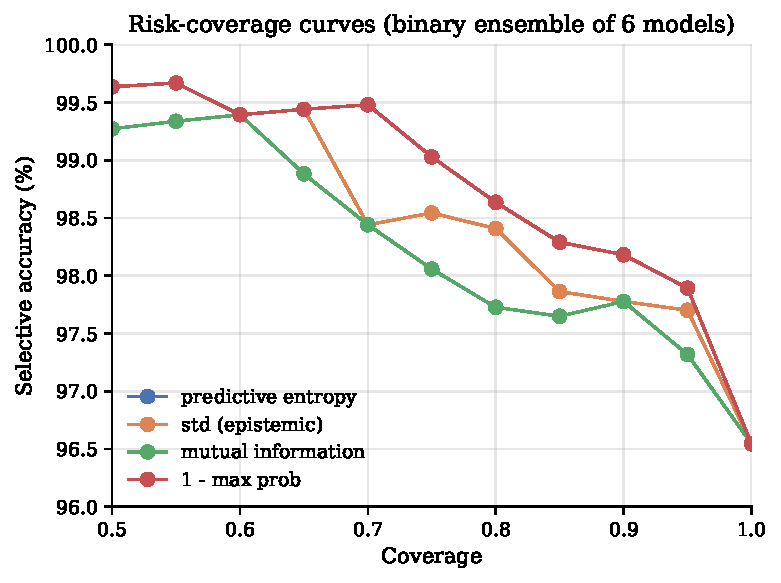
\includegraphics[width=0.75\linewidth]{figures/fig_phase1_risk_coverage.pdf}
%   \caption{Selective accuracy at varying coverage. At 90\% coverage,
%   accuracy reaches 98.18\%; at 50\%, 99.64\%.}
%   \label{fig:phase1-rc}
% \end{figure}
%
% - Best uncertainty signals are predictive entropy and 1 - max(p);
%   mutual information underperforms.
% - At 90\% coverage, the system improves from 96.55 to 98.18\%, freeing the
%   clinician to focus on the hardest 10\%.

\section{Lessons from Phase 1}
% - Test set augmentation in the bachelor pipeline inflated accuracy by
%   ~1-2 pp; fixing it cost some "headline numbers" but is correct.
% - 5 of 6 models statistically indistinguishable — the bachelor framing
%   ("model X is better than Y by 0.X pp") is not supported by the data.
% - Calibration is reasonable already, no severe over-confidence.
% - The remaining gap to clinical-grade reliability lies in (a) what to
%   do when the model is wrong but confident, and (b) extending the
%   analysis from binary to the actual 5-stage clinical task. These are
%   addressed in Phase 2 and Phase 3 respectively.
